\begin{savequote}[8cm]
Well, you shouldn’t believe
everything you read in the papers.

  \qauthor{--- Hans Bethe \textit{F. Reienes, Nobel Lecture 1995}}

\end{savequote}

\chapter{\label{ch:nu-theo}The Theory of Neutrinos}
\minitoc
The main goal of neutrino experiments is to measure all neutrino properties, including the mass, mixing angles, and the CP violation parameter, $\dcp$. 
The mixing angles and $\dcp$ fully describes neutrino oscillation, while the mass is the reason why neutrino oscillation occurs.
Hence, these parameters will be better illustrated in Sec.~\ref{sec:oscillation} in the context of the theoretical framework of neutrino oscillation.
As only products from neutrino interactions are detected in experiments, achieving this goal requires a good understanding of neutrino interactions.
Hence, a brief overview of neutrino interactions is given in Sec.~\ref{sec:interaction}.

\section{Oscillation}
\label{sec:oscillation}
Neutrinos come in three flavours: the electron neutrino ($\nu_e$), the muon neutrino ($\nu_\mu$), and the tau neutrino ($\nu_\tau$).
The different flavours of neutrinos will only produce the corresponding lepton in weak interactions, so they are eigenstates of the weak interaction.
However, neutrinos propagate through space as mass eigenstates, $\nu_1$, $\nu_2$, and $\nu_3$.
The reason for neutrino oscillation to occur is twofold.
One is because the mass eigenstates do not have a simple one-to-one correspondence with the weak eigenstates. 
They are superpositions of the weak eigenstates.
The other reason is that these mass eigenstates have different masses.
Neutrinos are created as flavour eigenstates in weak interactions, but they propagate as a linear combination of mass eigenstates, which propagate with different phase velocities due to their different masses.
Hence, throughout the propagation, the linear combination of mass eigenstates continually changes, leading to a varying superposition of flavour eigenstates, and thus, neutrino oscillation.

To be more specific, the matrix describing the mixing of mass eigenstates into flavour eigenstates is the PMNS matrix.
It is conventionally parametrised as 
\begin{equation}
U_{\text{PMNS}} = 
\begin{pmatrix}
1 & 0 & 0 \\
0 & c_{23} & s_{23} \\
0 & -s_{23} & c_{23}
\end{pmatrix}
\begin{pmatrix}
c_{13} & 0 & s_{13} e^{-i\dcp} \\
0 & 1 & 0 \\
-s_{13} e^{i\dcp} & 0 & c_{13}
\end{pmatrix}
\begin{pmatrix}
c_{12} & s_{12} & 0 \\
-s_{12} & c_{12} & 0 \\
0 & 0 & 1
\end{pmatrix},
\end{equation}
where $c_{ij} = \cos\theta_{ij}$ and $s_{ij} = \sin\theta_{ij}$, and $\dcp$ is the CP violation phase.
The angles $\theta_{ij}$ are the mixing angles. 
Using the PMNS matrix, the flavour eigenstates can be expressed in terms of the mass eigenstates as 
\begin{equation}
\begin{pmatrix}
\nu_e \\
\nu_\mu \\
\nu_\tau
\end{pmatrix}
=
U_{\text{PMNS}}
\begin{pmatrix}
\nu_1 \\
\nu_2 \\
\nu_3
\end{pmatrix}.
\end{equation}
The derivations of the following results can be obtained readily with pen and paper, so 
to keep a close focus on the development of the theoretical idea, detailed derivations are not included here. 
Due to the small neutrino masses, a mass eigenstate with mass $m_i$ acquires the following phase approximately:
\begin{equation}
  \ket{\nu_i(L)} = e^{-i \frac{m_i^2 L}{2E}} \ket{\nu_i(0)},
\end{equation}
after travelling a distance $L$ with energy $E$.
Hence, the probability that a neutrino of flavour $\alpha$ created at the source is detected as a neutrino of flavour $\beta$ after travelling a distance $L$ is given by
\begin{align}
  P_{(\alpha \to \beta)} &= \left|\braket{\nu_\beta | \nu_\alpha(L)} \right|^2 = \left| \sum_i U_{\alpha i} U^*_{\beta i} e^{-i \frac{m_i^2 L}{2E}} \right|^2 \\
  &= \delta_{\alpha\beta} - 4 \sum_{i>j} \text{Re} \bigl( U_{\alpha i} U^*_{\beta i} U^*_{\alpha j} U_{\beta j} \bigr) \,\sin^2 \!\Bigl( \frac{\Delta m^2_{ij} L}{4E} \Bigr) \\
  &\quad + 2 \sum_{i>j} \text{Im} \bigl( U_{\alpha i} U^*_{\beta i} U^*_{\alpha j} U_{\beta j} \bigr) \,\sin \!\Bigl( \frac{\Delta m^2_{ij} L}{2E} \Bigr),
\end{align}
where $\delta_{\alpha\beta}$ is the Kronecker delta, $U_{\alpha i}$ is the element of the PMNS matrix, and $\Delta m^2_{ij} = m_i^2 - m_j^2$.
This result shows that the oscillation probability depends on the mixing angle through the PMNS matrix elements and on the mass difference and neutrino energy through the sine terms.
For brevity, the dependence on the sine terms can be characterised by a phase angle,
\begin{equation}
  \label{eq:osc-phase}
  \Delta_{ij} = \frac{\Delta m^2_{ij} L}{2E} \approx 1.27 \frac{\Delta m^2_{ij} [\text{eV}^2] L [\text{km}]}{E [\text{GeV}]},
\end{equation}
where the oscillation is maximal when $\Delta_{ij} = \pi / 2$.
These results can be used to better understand how the various parameters are measured in different types of neutrino experiments.
The different sensitivities of these experiments arise from the relatively large differences in both the mixing angles and the mass differences.
The latest values for the neutrino parameters based on Ref.~\cite{Capozzi:2021fjo,ParticleDataGroup:2024cfk} are provided in Table~\ref{tab:neutrino-parameters}, which shows that the magnitude of $\delmtwoo$ is much smaller than that of $\delmthro$.
Unlike the CKM matrix, where all mixing angles are small, only $\theta_{13}$ is small here, while the other two angles are considerably larger, giving rise to significant mixing.

\begin{table}[h]
  \centering
  \begin{tabular}{c|c|c}
    Parameter & Value & Sensitive Experiment\\
    \hline
    \hline
    $\Delta m^2_{21}~(\text{eV}^2)$ & $7.36^{+0.16}_{-0.15} \times 10^{-5}$ & Reactor and solar \\
    $|\Delta m^2_{31}|~(\ev^2)$ & $2.448^{+0.023}_{-0.031} \times 10^{-3}$ & Atmospheric \\
    $\theta_{12}$ ($^\circ$) & $33.40^{+0.80}_{-0.82}$ & Reactor and solar \\
    $\theta_{23}$ ($^\circ$)       & $42.4^{+1.0}_{-0.9}$ & Atmospheric\\
    $\theta_{13}$ ($^\circ$)       & $8.59^{+0.13}_{-0.12}$ & Reactor and solar \\
    $\dcp$ ($^\circ$) & $223^{+32}_{-23}$   & Accelerator and atmospheric \\
    \hline
  \end{tabular}
  \caption{The latest values for the neutrino parameters.}
  \label{tab:neutrino-parameters}
\end{table}

\subsection{Atmospheric neutrinos}
Atmospheric neutrinos are mostly muon neutrinos produced from the decay of mesons created by cosmic rays interacting with the atmosphere.
The neutrino energy is typically of the order of $1~\gev$, while the distance travelled ranges from $O(10^2)$ to $O(10^4)~\km$.
Substituting these numbers into Eq.~\ref{eq:osc-phase}, $\Delta_{23}$ is of the order of $O(10^{-2})$ to $O(1)$, whereas $\Delta_{21}$ is of the order of $O(10^{-3})$ to $O(10^{-1})$.
Hence, oscillation is much more prominent in the $\nu_\mu \to \nu_\tau$ channel than in the $\nu_\mu \to \nu_e$ channel.
This is why atmospheric neutrino experiments are sensitive to $\theta_{23}$ and $\Delta m^2_{32}$, sometimes referred to as the atmospheric mixing angle and mass difference, respectively.

\subsection{Reactor neutrinos}
Reactor neutrinos are mostly electron antineutrinos produced from nuclear fission in power plants.
Their energy is typically of the order of $1~\mev$.
Unlike atmospheric neutrino measurements, detectors can be placed at various locations to measure different parameters.
Thus, it is more convenient to discuss reactor neutrino oscillation by introducing the oscillation length variable given as:
\begin{equation}
  \label{eq:osc-length}
  L_{\text{osc}} = \frac{4\pi E}{\Delta m^2} = 2.48 \frac{E [\text{MeV}]}{\Delta m^2 [\text{eV}^2]} \text{m},
\end{equation}
which corresponds to one complete period of neutrino oscillation.
Substituting the reactor neutrino energy into Eq.~\ref{eq:osc-length}, one obtains $L_{\text{osc}} = O(10^2)~\km$ for $\delmtwoo$ and $L_{\text{osc}} = O(1)~\km$ for $\delmthro$. 
Hence, by placing detectors kilometres away from the power plants, reactor neutrino experiments offer the unique opportunity to measure $\theta_{13}$ and $\delmthro$, sometimes referred to as the reactor mixing angle and mass difference, respectively.
Additionally, placing detectors at about $O(100)~\km$ from the power plants allows measurements of $\delmtwoo$.

\subsection{Solar neutrinos}
Solar neutrinos are mostly electron neutrinos produced from nuclear fusion in the Sun.
Most solar neutrinos have energies below $1~\mev$, except those from $^8$B decay, which can reach $15~\mev$.
The distance travelled by solar neutrinos is of the order of $O(10^8)~\km$.
Substituting these values into Eq.~\ref{eq:osc-length}, one obtains $L_{\text{osc}} = O(10^4)~\m$ for $\delmtwoo$ and $L_{\text{osc}} = O(10^3)~\m$ for $\delmthro$.
Both are much smaller than the average distance travelled, so observing the clear oscillatory pattern (as in other neutrino experiments) would require knowing each neutrino’s travel distance and starting position with extremely high precision, which is beyond current detection capabilities.
Fortunately, the average oscillation result can still be measured by the total survival rate of electron neutrinos.

Beyond the usual neutrino oscillation, there is another important phenomenon in solar neutrino measurements: the Mikheyev–Smirnov–Wolfenstein (MSW) matter effect~\cite{Wolfenstein:1977ue,Mikheyev:1985zog}.
A detailed discussion of the MSW effect is beyond the scope of this thesis.
In short, the MSW effect modifies the mixing parameters due to the presence of electrons in matter.
This modification can enhance or suppress the oscillation probability depending on the mass difference and the electron density.
Roughly speaking, the required electron density is proportional to the mass difference squared and inversely proportional to the neutrino energy.
Hence, lower neutrino energy or a larger mass difference necessitates a higher electron density to modify the oscillation probability.
Because $\delmthro$ is considerably larger, for nearly all solar neutrino energies, the electron density in the Sun is insufficient to modify the mixing between $\nu_1$ and $\nu_3$ significantly.
As for the relatively smaller $\delmtwoo$, the electron density is high enough to substantially modify the mixing between $\nu_1$ and $\nu_2$ for the high-energy neutrinos from $^8$B decay.
The outcome for these high-energy electron neutrinos is a rearrangement of their mass-eigenstate composition such that, upon leaving the Sun’s surface, they are mostly $\nu_2$, a considerably greater fraction than in the unmodified scenario for the low-energy electron neutrinos.
The MSW effect is seen when different experiments measure solar neutrinos at different energies and observe varying electron-neutrino survival rates.
Hence, the absolute survival rates are particularly sensitive to $\theta_{12}$, which is often referred to as the solar mixing angle. 

\subsection{Accelerator neutrinos}
In accelerator neutrino experiments, there is relatively greater flexibility than in other types of neutrino experiments because both the neutrino source and the detector can be designed to optimise oscillation studies.
This section uses T2K as an example, but the underlying principles apply to all LBL experiments.
More details about the T2K experiment are presented in Chapter~\ref{ch:t2k}.

Neutrinos are produced in accelerators by bombarding protons onto a target (carbon in T2K), creating numerous mesons.
The charged mesons can be steered to point in the required direction using sophisticated magnetic horns.
Besides directionality, the magnetic horns can also select mesons of a desired charge.
For instance, positive (negative) pions can be focused if a beam of muon (anti)neutrinos is needed.
It is this control over the neutrino source that enables accelerator experiments to measure $\delta_{CP}$.
Since the neutrino energy from meson decay depends on the emission angle, varying the angle between the detector and the beam direction yields different energy distributions.
T2K places its detectors $2.5^\circ$ off-axis to obtain a neutrino beam with a narrow energy peak at about $0.6~\gev$.
According to Eq.~\ref{eq:osc-phase}, for maximal oscillation with the larger mass difference (i.e.\ $\delmthro \approx 2.5 \times 10^{-3}~\ev^2$), the far detector should be placed around $300$~km from the source.
Hence, accelerator measurements are sensitive to $\theta_{13}$.
Furthermore, by analysing muon neutrino disappearance, accelerator experiments can also measure $\theta_{23}$ and $\delmthrt$.
By analysing oscillations in neutrino and antineutrino modes, T2K can extract a best-fit value of $\delta_{CP}$ that describes the observed data~\cite{T2K:2019bcf}.
However, the current measurement is severely limited by statistics and thus suffers large uncertainties.
Due to the significant increase in the fiducial volume of Hyper-K, statistics are expected to increase significantly, and reducing systematic uncertainties proportionally will be paramount for fully exploiting that potential.
This leads naturally to the discussion of one of the major sources of systematic uncertainty in neutrino experiments: neutrino interactions.

\section{Interaction}
\label{sec:interaction}
The underlying theory for neutrino oscillation is straightforward, and the parameters to be measured are clear, but the experimental determination of these parameters is challenging.
Due to the weak interaction of neutrinos, they cannot be detected directly.
All neutrino measurements are based on detecting the particles produced in neutrino interactions.
Hence, to extract the desired neutrino oscillation parameters with high precision, a good understanding of neutrino interactions is crucial.
This chapter provides the basic understanding of neutrino interactions necessary for interpreting the analyses presented in the subsequent chapters.

\subsection{$\nu$-quark}
The most fundamental interaction between a neutrino and matter is the weak interaction between the neutrino and a quark, whose Feynman diagrams are shown in Fig.~\ref{fig:nu-q-feyn}.

\begin{figure}[h]
  \centering
  \begin{subfigure}[b]{0.45\textwidth}
    \centering
    \begin{tikzpicture}
      \begin{feynman}
        \vertex (a) {\(\nu_\ell\)};
        \vertex [right=of a] (b);
        \vertex [right=of b] (c) {\(\ell\)};
        \vertex [below=of b] (d);
        \vertex [left=of d] (e) {\(q\)};
        \vertex [right=of d] (f) {\(q'\)};
        
        \diagram* {
          (a) -- [fermion] (b) -- [fermion] (c),
          (b) -- [boson, edge label=\(W\)] (d),
          (e) -- [fermion] (d) -- [fermion] (f),
        };
      \end{feynman}
    \end{tikzpicture}
    \caption{Charge current interaction.}
    \label{fig:cc-interaction}
  \end{subfigure}
  \hfill
  \begin{subfigure}[b]{0.45\textwidth}
    \centering
    \begin{tikzpicture}
      \begin{feynman}
        \vertex (a) {\(\nu_\ell\)};
        \vertex [right=of a] (b);
        \vertex [right=of b] (c) {\(\nu_\ell\)};
        \vertex [below=of b] (d);
        \vertex [left=of d] (e) {\(q\)};
        \vertex [right=of d] (f) {\(q\)};
        
        \diagram* {
          (a) -- [fermion] (b) -- [fermion] (c),
          (b) -- [boson, edge label=\(Z\)] (d),
          (e) -- [fermion] (d) -- [fermion] (f),
        };
      \end{feynman}
    \end{tikzpicture}
    \caption{Neutral current interaction.}
    \label{fig:nc-interaction}
  \end{subfigure}
  \caption{Feynman diagrams for neutrino interactions with a quark.}
  \label{fig:nu-q-feyn}
\end{figure}
More specifically, the interaction shown in Fig.~\ref{fig:cc-interaction} is mediated by the $W$ boson, and the neutrino is converted into a charged lepton, while Fig.~\ref{fig:nc-interaction} is mediated by the $Z$ boson, and the neutrino remains a neutrino.
The former is the charged current (CC) interaction, while the latter is the neutral current (NC) interaction.
Following the Feynman diagram, it is straightforward to write down the amplitude for the interaction.
The amplitude for the CC interaction is given by:
\begin{equation}
  \mathcal{M}_{\text{CC}} = \frac{g^2}{2} \bar{u}_\ell(p') \gamma^\mu (1 - \gamma^5) u_\nu(p) \frac{-i g_{\mu\nu}}{q^2 - M_W^2} \bar{u}_q(k') \gamma^\nu (1 - \gamma^5) u_q(k),
\end{equation}
where $g$ is the weak coupling constant, $u_\ell$ and $u_\nu$ are the spinors for the outgoing lepton and incoming neutrino respectively, $u_q$ are the spinors for the quarks, $q$ is the momentum transfer, and $M_W$ is the mass of the $W$ boson.
Due to confinement, this interaction does not occur freely in nature.
Instead, this interaction occurs only when the neutrino has sufficiently high energy to probe inside the nucleon and interact with the quarks.
The product quark will hadronise, producing a jet of particles.
This type of interaction is referred to as deep inelastic scattering (DIS).
DIS is highly complicated and not so relevant for this thesis, so it will not be discussed further.
More details can be found in reviews such as Ref.~\cite{SajjadAthar:2022pjt}.

\subsection{$\nu$-nucleon}
At the T2K beam energy, most neutrinos do not have enough energy to probe within the nucleon but rather interact with the nucleon as a whole.
Depending on the specific neutrino energy, the interaction can be classified as quasi-elastic (QE), resonance, or deep inelastic scattering (DIS).

\subsubsection{QE}
Although at the quark level the interaction appears the same as in Fig.~\ref{fig:nu-q-feyn}, the interacted quark cannot be treated as independent but rather as part of a nucleon.
Hence, the effective $\nu$-nucleon interaction Feynman diagram is shown in Fig.~\ref{fig:nu-n-feyn}.

\begin{figure}[h]
  \centering
  \begin{subfigure}[b]{0.45\textwidth}
    \centering
    \begin{tikzpicture}
      \begin{feynman}
        \vertex (a) {\(\nu_\ell\)};
        \vertex [right=of a] (b);
        \vertex [right=of b] (c) {\(\ell\)};
        \vertex [below=of b] (d);
        \vertex [left=of d] (e) {\(N\)};
        \vertex [right=of d] (f) {\(N'\)};
        
        \diagram* {
          (a) -- [fermion] (b) -- [fermion] (c),
          (b) -- [boson, edge label=\(W\)] (d),
          (e) -- [fermion] (d) -- [fermion] (f),
        };
      \end{feynman}
    \end{tikzpicture}
    \caption{Charge current interaction.}
    \label{fig:cc-interaction-n}
  \end{subfigure}
  \hfill
  \begin{subfigure}[b]{0.45\textwidth}
    \centering
    \begin{tikzpicture}
      \begin{feynman}
        \vertex (a) {\(\nu_\ell\)};
        \vertex [right=of a] (b);
        \vertex [right=of b] (c) {\(\nu_\ell\)};
        \vertex [below=of b] (d);
        \vertex [left=of d] (e) {\(N\)};
        \vertex [right=of d] (f) {\(N\)};
        
        \diagram* {
          (a) -- [fermion] (b) -- [fermion] (c),
          (b) -- [boson, edge label=\(Z\)] (d),
          (e) -- [fermion] (d) -- [fermion] (f),
        };
      \end{feynman}
    \end{tikzpicture}
    \caption{Neutral current interaction.}
    \label{fig:nc-interaction-n}
  \end{subfigure}
  \caption{Feynman diagrams for neutrino interactions with a nucleon.}
  \label{fig:nu-n-feyn}
\end{figure}
The leptonic current remains the same, but the hadronic current is now a nucleon current instead of a quark current.
Hence, the hadronic current is much more complicated, comprising several form factors that parametrise our understanding of the nucleon structure.
For instance, the amplitude for the CC interaction in Fig.~\ref{fig:cc-interaction-n} is given by:
\begin{align}
  \mathcal{M}_{\text{CC}} = \frac{G_F}{\sqrt{2}} \,\bar{u}_\ell(p')\,\gamma^\mu (1 - \gamma^5)\,u_\nu(p) \\
  \times \,\bar{u}_N(k')\,\left[ F_1(q^2)\,\gamma_\mu + F_2(q^2)\,\frac{i\,\sigma_{\mu\nu}\,q^\nu}{2M} + F_A(q^2)\,\gamma_\mu\,\gamma^5 + F_P(q^2)\,\frac{q_\mu\,\gamma^5}{m_\pi} \right]\,u_N(k),
\end{align}
where $G_F$ is the Fermi constant, $M$ is the nucleon mass, $m_\pi$ is the pion mass, and the hadronic current is parametrised by the form factors, $F_1$, $F_2$, $F_A$, and $F_P$.
More details can be found in Ref.~\cite{LlewellynSmith:1978te}.
It is important to note that $F_1$ and $F_2$ are the vector form factors, which can be extracted from electron scattering measurements, and $F_P$ is the pseudoscalar form factor, which can be related to $F_A$, the axial form factor, through the Partially Conserved Axial Current (PCAC) hypothesis.
Hence, the axial form factor is unique to neutrino experiments and can only be extracted from past measurements.
Fig.~\ref{fig:cc0pi} shows an event display of a candidate $\cczpi$ event, likely a QE event, in the upgraded ND280 during the beam run in June 2024.

\begin{figure}[!htb] 	
    \centering 		
    \includegraphics[width=\sgfigwid\textwidth]{figures/cc0pi.png}
    \caption{\label{fig:cc0pi} A $\cczpi$ candidate event in upgraded ND280, where the long track is the primary muon and the short track is the primary proton.} 
\end{figure}

\subsubsection{Resonance}
When the neutrino energy is high enough to excite the nucleon to a higher energy state (e.g.\ $\Delta(1232)$), the interaction is classified as a resonance interaction.
The excited nucleon decays to produce a pion. 
Hence, resonance modelling is sometimes called single pion production modelling.
One of the most common models used today is the Berger–Sehgal model, which is an improvement on the earlier Rein–Sehgal model by accounting for the effect of the lepton mass.
The Rein–Sehgal model is based on the approximate relativistic quark model in Ref.~\cite{Feynman:1971wr}.
Subsequent developments, such as the MK model~\cite{Kabirnezhad:2017jmf,Kabirnezhad:2020wtp,Kabirnezhad:2022znc}, provide more sophisticated calculations.

Fig.~\ref{fig:cc1pi} shows an event display of a candidate $\ccopi$ event, likely a resonance event, in the upgraded ND280 during the beam run in June 2024.

\begin{figure}[!htb] 	
    \centering 		
    \includegraphics[width=\sgfigwid\textwidth]{figures/shortME.png}
    \caption{\label{fig:cc1pi} A $\ccopi$ candidate event in upgraded ND280, where the long track is the primary muon and the V-shaped track is identified as a pion track by the short delayed track, identified as the Michel electron, attached to its end.} 
\end{figure}

\subsection{$\nu$-nucleus}
\label{sec:nuint-nucleus}
Modern neutrino experiments use heavier elements, such as hydrocarbon and argon, to increase event rates.
This further complicates the neutrino interaction.
In the simplest case (relatively high neutrino energy), the Impulse Approximation (IA) can be applied.
The neutrino sees each nucleon as independent, so the interaction reduces to the $\nu$-N interaction.
Even in this simplest case, the presence of the nuclear medium still affects the interaction in two ways: the initial state (IS) effect and the final state interaction (FSI).

As the neutrino energy decreases, IA is no longer valid, and the nucleus can only be resolved as a whole.
In this case, Random Phase Approximation (RPA) corrections are needed.
Interested readers can refer to Ref.~\cite{SajjadAthar:2022pjt} for more details.
Instead, the two nuclear effects are elaborated below.

\subsubsection{Initial state}
Nuclear effects manifest in two ways.
Firstly, the nucleon in the interaction is in a bound state, meaning it cannot have arbitrary energy and momentum as a free nucleon would.
Instead, the nucleon’s energy distribution is parameterised by the so-called Spectral Function (SF).
The simplest form of SF is the Fermi gas model, which treats nucleons as a Fermi gas.
Hence, the nucleon momentum is filled up to the Fermi momentum, given by
\begin{equation}
    k_F = \bigl(3\pi^2 \rho/2\bigr)^{1/3},
\end{equation}
where $\rho$ is the nuclear density, approximately $2.3\times 10^{-17}~\textrm{kg}/\m^3$, leading to a Fermi momentum of about $250~\mevc$.
This model oversimplifies the nuclear structure.
A more realistic approach is the local Fermi gas (LFG) model, which accounts for the varying nuclear density.
Further improvements include short-range correlations between nucleons, which increase the fraction at high momentum~\cite{Benhar:1994hw}.

\subsubsection{FSI}
\label{sec:nuint-fsi}
The second nuclear effect is the final state interaction (FSI).
Regardless of how the neutrino interacts with the nucleon, the products remain inside the nucleus and must propagate through the nuclear medium to be detected.
These interactions with the nuclear medium are classified as FSI.
They are more pronounced for hadrons than for leptons, as the latter are less likely to interact in the nuclear medium.
There are several types of FSI, including elastic scattering, charge exchange, and absorption.
\begin{enumerate}
  \item 
  Charge exchange (CEX) involves changing the charge of the participating particles; for example,
  \begin{equation}
      \pi^+ + n \rightarrow \pi^0 + p,
  \end{equation}
  or vice versa. This rescattering type is crucial for event topologies requiring the presence of a pion; depending on the signal pion’s charge, CEX could migrate events between signal and background. 

  \item 
  Inelastic scattering (INEL) is the case where the nucleus is left in an excited state after rescattering. This category applies only to situations where a single additional nucleon is emitted or knocked out after rescattering. Since it does not affect the number of pions, it will not convert a pionless topology into a pion-production topology. However, it can change the number of final-state nucleons and affect the kinematics of the leading particle.

  \item 
  Absorption (ABS) refers to processes where the pion is effectively absorbed. For instance, $\pi^+$ can interact with multiple nucleons, initially forming a baryon resonance that subsequently emits multiple nucleons rather than a pion. Thus, the $\pi^+$ no longer emerges from the nucleus.

  \item 
  Pion production (PIPD) can occur for energetic particles where an extra pion is generated through rescattering, for example:
  \begin{equation}
      p + p \rightarrow p + n + \pi^+.
  \end{equation}
  Such an interaction significantly alters the event topology, adding an extra pion.
\end{enumerate}

\subsubsection{Transverse Kinematic Imbalance}
\label{sec:nuint-tki}
Due to the heavy target nucleus in current neutrino experiments, nuclear effects are almost inextricable from conventional single-particle kinematic measurements.
This greatly impedes model development because nuclear effects can mimic different underlying $\nu$-N processes.
For instance, if the proton from a QE $\nu$-N interaction has sufficient energy to produce an additional pion during FSI, that pion may emerge from the nucleus.
Thus, a QE event could mimic resonance production.
Hence, accurate descriptions of nuclear effects are crucial to reduce model systematic uncertainties.

To gain insights into nuclear effects, observables that are sensitive to these effects must be measured.
Transverse Kinematic Imbalance (TKI) variables are exactly such observables~\cite{Lu:2015hea, Lu:2015tcr}.
The TKI variables are illustrated in Fig.~\ref{fig:stki}.

\begin{figure}[!htb] 	
    \centering 		
    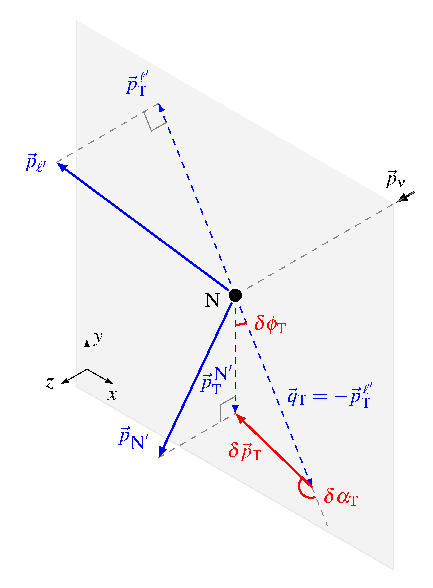
\includegraphics[width=0.35\textwidth]{figures/stki.eps}
    \caption{\label{fig:stki} Schematic illustration of the TKI variables. Diagram taken from Ref.~\cite{Lu:2015tcr}.} 
\end{figure}

In the simplest case, there are only two final particles after the neutrino–nucleon interaction: a muon and a proton. 
Without nuclear effects, these two particles should have momenta of equal magnitude but opposite direction in the plane transverse to the neutrino beam.
The TKI variables quantify the deviation from this ideal scenario, thereby probing nuclear effects. 
Because of the initial state (IS), the nucleon’s momentum distribution causes the sum of the muon and proton transverse momenta to deviate from zero, quantified by $\dpt$, and their directions need not be precisely opposite, quantified by $\dphit$.
Moreover, if the nucleus is initially at rest and no additional particles (beyond the muon and proton) are knocked out, the nucleon initial momentum $\pn$ can be estimated with an $\mathcal{O}(20\%)$ correction~\cite{Yang:2023dxk} following methods in Refs.~\cite{Furmanski:2016wqo, Lu:2019nmf}. 
Hence, $\dpt$ and $\pn$ serve as good probes of IS models.
While FSI tends to smear these distributions, the general shape and peak location mainly reflect the IS model.
Since most IS models assume no preferred direction for nucleon motion, one expects a uniform distribution in $\dat$, the angle between the initial nucleon momentum and the lepton momentum in the transverse plane.
Any deviation from flatness in $\dat$ is thus attributed to FSI, making it an excellent probe of FSI. 

In pion-production events, a double-transverse variable, $\dptt$, can be constructed by projecting $\vecdpt$ onto the axis perpendicular to the lepton scattering plane, defined by $\vecpl$ and $\vecpnu$ (see Fig.~\ref{fig:dtki}).
\begin{figure}[!htb] 	
    \centering 		
    \includegraphics[width=0.35\textwidth]{figures/dptt.pdf}
    \caption{\label{fig:dtki} Schematic illustration of the double TKI variable. Diagram taken from Ref.~\cite{T2K:2021naz}.} 
\end{figure}

In the absence of nuclear effects, $\dptt$ should be zero.
Its distribution width reveals the role of nuclear effects in pion production~\cite{MINERvA:2020anu, T2K:2021naz}.
Analogous variables, $\dptx$ and $\dpty$, have been proposed and studied in MINERvA~\cite{MINERvA:2019ope} for pionless channels.
Additionally, Refs.~\cite{Lu:2015tcr,Hamacher-Baumann:2020ogq} suggest using $\dptt$ to isolate a hydrogen sample.  
More details on hydrogen selections will be given in Sec.~\ref{sec:mc-hydrogen}.

There has been a wealth of TKI-based measurements from multiple neutrino experiments, including T2K~\cite{T2K:2018rnz, T2K:2021naz}, MINERvA~\cite{MINERvA:2018hba, MINERvA:2019ope, MINERvA:2020anu, MINERvA:2021csy}, and MicroBooNE~\cite{MicroBooNE:2022emb, MicroBooNE:2023cmw, MicroBooNE:2023tzj, MicroBooNE:2023wzy, MicroBooNE:2024tmp}.
Because the TKI concept applies equally to electron scattering, experiments such as CLAS~\cite{CLAS:2021neh} have also produced TKI measurements, demonstrating the wide applicability of TKI.
